% =========================================================================== %
% One Day Tutorial
% =========================================================================== %

\ifx\wholebook\relax\else
  \documentclass[a4paper,10pt,twoside]{book}
  %=============================================================================%
% Common things, settings, packages to include
%=============================================================================%

\usepackage{graphicx}
\usepackage{color}
\usepackage{makeidx}
\usepackage{ifpdf}
\usepackage{verbatim}

% --------------------------------------------------------------------------- %
% Setting up stuff depeding on output format
% --------------------------------------------------------------------------- %

\ifpdf
  % special settings for pdf mode
  \usepackage[colorlinks]{hyperref}
  \usepackage{courier}
  
  \hypersetup{
    colorlinks,
    linkcolor=darkblue,
    citecolor=darkblue,
    pdftitle={The Eclipse Scout Book},
    pdfauthor={The Scout Community},
    pdfkeywords={Enterprise Framework, Eclipse, Java, Client-Side, Rich Client, Web Client, Mobile},
    pdfsubject={Computer Science}
  }
  
  \usepackage{caption}
  \captionsetup{margin=10pt,font=small,labelfont=bf}
\else
  % special stuff for html mode
  \usepackage[tex4ht]{hyperref}
\fi

% --------------------------------------------------------------------------- %
% Setting up printing range
% --------------------------------------------------------------------------- %

\parindent 1cm
\parskip 0.2cm
\topmargin 0.2cm
\oddsidemargin 1cm
\evensidemargin 0.5cm
\textwidth 15cm
\textheight 21cm

% --------------------------------------------------------------------------- %
% Setting up listings
% --------------------------------------------------------------------------- %

\usepackage{listings}
 
\definecolor{darkviolet}{rgb}{0.5,0,0.4}
\definecolor{darkgreen}{rgb}{0,0.4,0.2} 
\definecolor{darkblue}{rgb}{0.1,0.1,0.9}
\definecolor{darkgrey}{rgb}{0.5,0.5,0.5}
\definecolor{lightblue}{rgb}{0.4,0.4,1}
\definecolor{lightgray}{rgb}{0.97,0.97,0.97}

\renewcommand{\lstlistlistingname}{List of Listings}

% general settings
\lstset{
  basicstyle=\small\ttfamily,
  columns=fullflexible,
  breaklines=true,
  breakindent=10pt,
  prebreak=\mbox{{\color{blue}\tiny$\searrow$}},
  postbreak=\mbox{{\color{blue}\tiny$\rightarrow$}},
  showstringspaces=false,
  backgroundcolor=\color{lightgray}
}

% settings for xml files
\lstdefinelanguage{xml}
{
  commentstyle=\color{darkgrey}\upshape,
  morestring=[b]",
  morestring=[s]{>}{<},
  morecomment=[s]{<?}{?>},
  stringstyle=\color{black},
  identifierstyle=\color{darkblue},
  keywordstyle=\color{cyan},
  morekeywords={xmlns,name,point,factory,class}% list your attributes here
}

% settings for ini files
\lstdefinelanguage{ini}
{
  morecomment=[f][\color{darkgrey}\upshape][0]\#, % # is comment iff it's the first char on the line
  stringstyle=\color{black}
}

% default settings (for java files)
\lstset{
  language=Java,
  emphstyle=\color{red}\bfseries,
  keywordstyle=\color{darkviolet}\bfseries,
  commentstyle=\color{darkgreen},
  morecomment=[s][\color{lightblue}]{/**}{*/},
  stringstyle=\color{darkblue},
}

% --------------------------------------------------------------------------- %
% cross reference macros
% --------------------------------------------------------------------------- %
\newcommand{\applabel}[1]{\label{apx:#1}}
\newcommand{\chalabel}[1]{\label{cha:#1}}
\newcommand{\seclabel}[1]{\label{sec:#1}}
\newcommand{\lstlabel}[1]{\label{lst:#1}}
\newcommand{\figlabel}[1]{\label{fig:#1}}
\newcommand{\tablabel}[1]{\label{tab:#1}}

\newcommand{\appref}[1]{Appendix~\ref{apx:#1}}
\newcommand{\charef}[1]{Chapter~\ref{cha:#1}\xspace}
\newcommand{\secref}[1]{Section~\ref{sec:#1}}
\newcommand{\lstref}[1]{Listing~\ref{lst:#1}\xspace}
\newcommand{\figref}[1]{Figure~\ref{fig:#1}\xspace}
\newcommand{\tabref}[1]{Table~\ref{tab:#1}\xspace}

% --------------------------------------------------------------------------- %
% graphics paths
% --------------------------------------------------------------------------- %
\graphicspath{
  {figures/}
  {Introduction/figures/}
}

%=============================================================================%

  \pagestyle{headings}
  \graphicspath{{figures/} {../figures/}}
  \begin{document}
  \sloppy
\fi

% --------------------------------------------------------------------------- %
\chapter{A Larger Example}
\chalabel{large_example}

In this chapter we will create the ''My Contacts'' Scout application.
This small\footnote{
Small in comparison with real world application. But significantly larger and complexer than the ''Hello World'' application of \charef{helloworld}.
} application covers additional aspects of the Eclipse Scout framework. 
The presented demo application borrows heavily from a Scout tutorial published in 2012 the German \textit{Java Magazin}\footnote{
Java Magazin 7.12: \url{https://jaxenter.de/magazines/JavaMagazin72012}.
} 
for the Scout release 3.8 (Juno).
Compared to the 2012 tutorial, the version presented in this chapter has been slightly polished and updated to the Scout release 3.9 (Kepler).

Specifically, we will build an outline based Scout application featuring a navigation tree and pages to present information in tabular form. 
In addition, the application also shows how to work with forms to enter and/or update data, menus and context menus. 
On the server side, we show how to work with databases, how to use logging in Scout applications and how to include standard Java libraries available in JAR files. 

The chapter is organized as follows.
In the first section, the finished demo application is explained from the user perspective. 
The remaining sections focus on the individual steps to implement the ''My Contacts'' application. 
To follow the description of the implementation the reader is assumed to be familiar with the ''Hello World'' tutorial and the Scout SDK as described in \charef{tooling}. 

% --------------------------------------------------------------------------- %
\section{The ''My Contacts'' Application}

The ''My Contacts'' application is a client server application to manage personal contacts. 
Persistece of entered data is achieved through a database backend. 

As social networking services\footnote{
Social networking services in Wikipedia: \url{http://en.wikipedia.org/wiki/Social_network_service}
} 
such as Facebook, LinkedIn or Xing are widely used, the application also provides an example integration with the LinkedIn\footnote{
\url{http://www.linkedin.com/}
} 
plattform. 
The implemented integration allows to download the personal contacts into the local database. 
In the local database it is possible to mix persons entered manually with contact data downloaded from LinkedIn. 

\begin{figure}
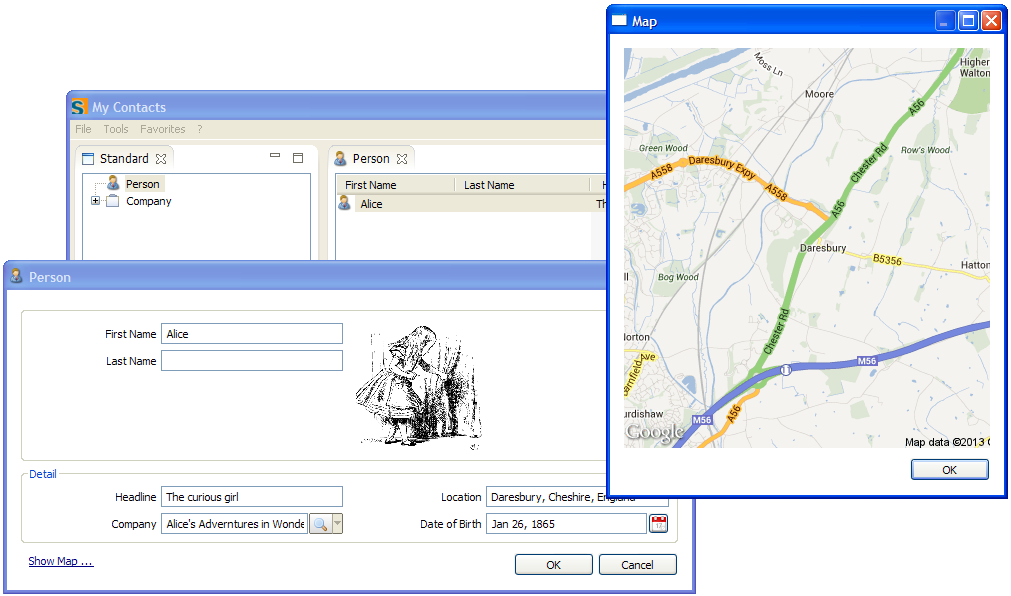
\includegraphics[width=14cm]{my_contacts_swt.png} 
\caption{The SWT client of the ''My Contacts'' application. }
\figlabel{my_contacts_swt}
\end{figure}

After starting the Scout server application a client application may be started that then connects to the server. 
In \figref{my_contacts_swt} the SWT desktop client is shown. 
In the background, the main application window is visible showing a navigation tree on the left hand side. 
On the right side, a table holds the elements corresponding to the selected tree node. 
Using an edit context menu on the selected table row, a form to edit the releant data may be opened as shown in the example screenshot for 'Alice'. 
Clicking on the link 'Show Map ...' in the person form opens the person's location information in a map form using the data provided by Google Maps Image API\footnote{
The Google Maps Image APIs: \url{https://developers.google.com/maps/documentation/imageapis/}.
}.

\begin{figure}
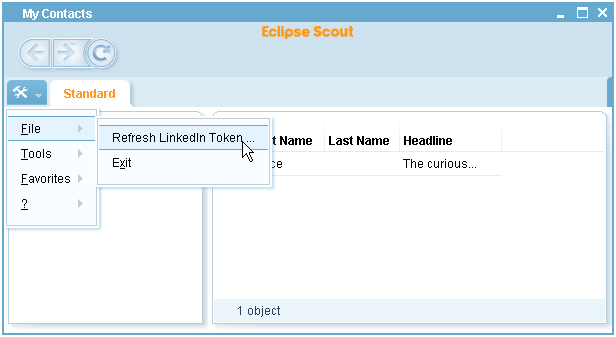
\includegraphics[width=9cm]{my_contacts_rayo_refresh.png} 
\caption{To refresh/generate an access token for reading LinkedIn contacts data select the menu shown in the screenshot. }
\figlabel{my_contacts_rayo_refresh}
\end{figure}

\begin{figure}
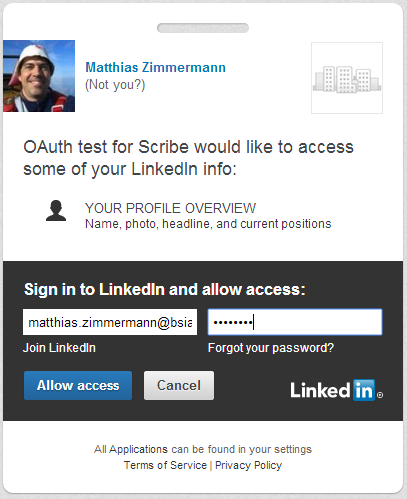
\includegraphics[width=7cm]{my_contacts_rayo_openauthurl.png} \hspace{5mm}
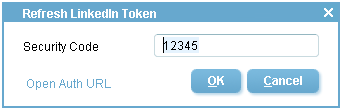
\includegraphics[width=7cm]{my_contacts_rayo_entercode.png}
\caption{To refresh/create the access token click on the provided 'Open Auth URL' link first (left). 
Then, the security code field is enabled and the user can fill in the security code provided on the LinkedIn web page. }
\figlabel{my_contacts_rayo_openauthurl}
\end{figure}

Before any LinkedIn data can be accessed from the ''My Contacts'' application an access token needs to be retrieved from LinkedIn. 
To obtain such a token use the \menu{Refresh LinkedIn Token ...} as shown in \figref{my_contacts_rayo_refresh}. 
This opens the refesh token form shown on the left side of \figref{my_contacts_rayo_openauthurl}. 

\begin{figure}
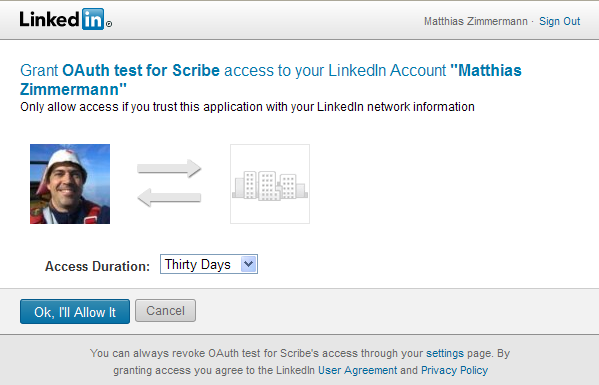
\includegraphics[width=7cm]{oauth_grant_access.png} \hspace{5mm}
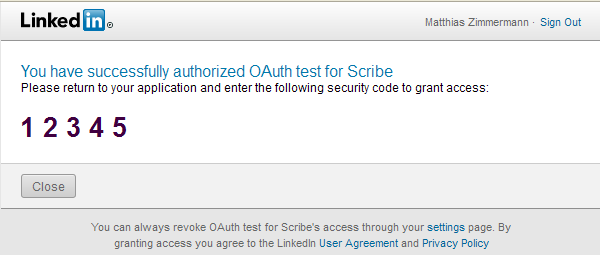
\includegraphics[width=7cm]{oauth_security_code.png} 
\caption{The LinkedIn granting dialog steps shown in a web browser. 
In the first step (right) confirm the access request, then the security code to create an access token is provided in the second step (left).
}
\figlabel{oauth_security_code}
\end{figure}

Clicking on the 'Open Auth URL' link then opens the granting page provided by LinkedIn shown on the left hand side of \figref{oauth_security_code}. 
After logging into your LinkedIn account\footnote{
Yes, for this use case you need a LinkedIn accout. But at least it's free and you will not need to provide very sensitive information such as a mobile phone number, a credit card number or a social security number. 
}
you can specify the desired access duration and confirm the ''OAuth test for Scribe'' access\footnote{
This is the name of the example code provided with the Scribe library that is used with the ''My Contacts'' application. 
} 
to your LinkedIn data.
If the authorization is successful, a security code as shown on the right side of \figref{oauth_security_code} is presented by LinkedIn. 
This code needs then to be entered into the \field{Security Code} as shown on the right side of \figref{my_contacts_rayo_openauthurl}. 
Then, click the \button{OK} to refersh the access token. 

\begin{figure}
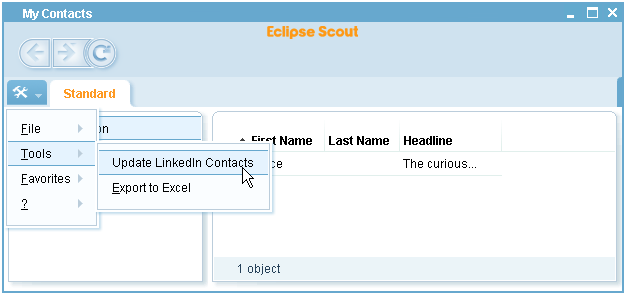
\includegraphics[width=9cm]{my_contacts_rayo_updatecontacts.png} \hspace{5mm}
\caption{Executing the 'Update LinkedIn Contacts for the first time imports the users LinkedIn contacts into the ''My Contacts'' application.}
\figlabel{my_contacts_rayo_updatecontacts}
\end{figure}

To import/update your LinkedIn contacts into your ''My Contacts'' application select the \menu{Update LinkedIn Contacts} as shown in \figref{my_contacts_rayo_updatecontacts}.
Once you have downloaded or entered a number of persons in your ''My Contacts'' application, try to get yourself familiar with the application's person table. 
This is one of the very powerful Scout widgets. 
Columns may be filtered, moved, hidden or sorted (including multi level sort) using the table header context menues \menu{Organize Columns...}  and \menu{Column Filter...}.

Editing and viewing of person data is available by the \contextmenu{Edit Person...} on a selected row.
To manually add a person use the context \contextmenu{New Person...} available on the table header or in the white area outside the displayed columns. 

\begin{figure}
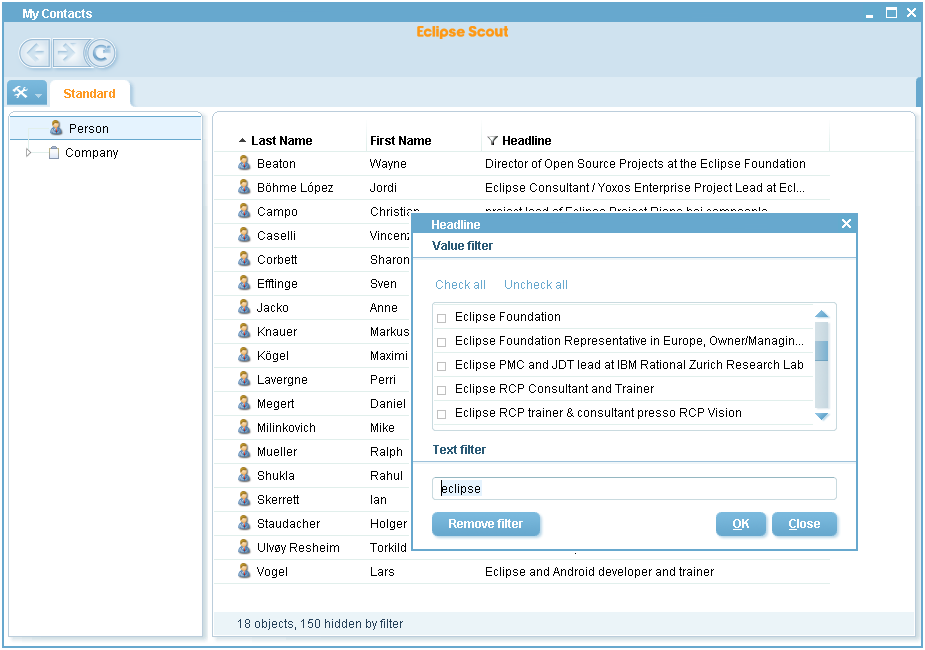
\includegraphics[width=14cm]{my_contacts_rayo_filteredcontacts.png} 
\caption{After importing the contacts from LinkedIn the data is shown in the person page. 
The filter applied on the headline column is indicated by the filter icon. In the front, the filter form shows the filter criterial 'Eclipse'.}
\figlabel{my_contacts_rayo_filteredcontacts}
\end{figure}

\begin{figure}
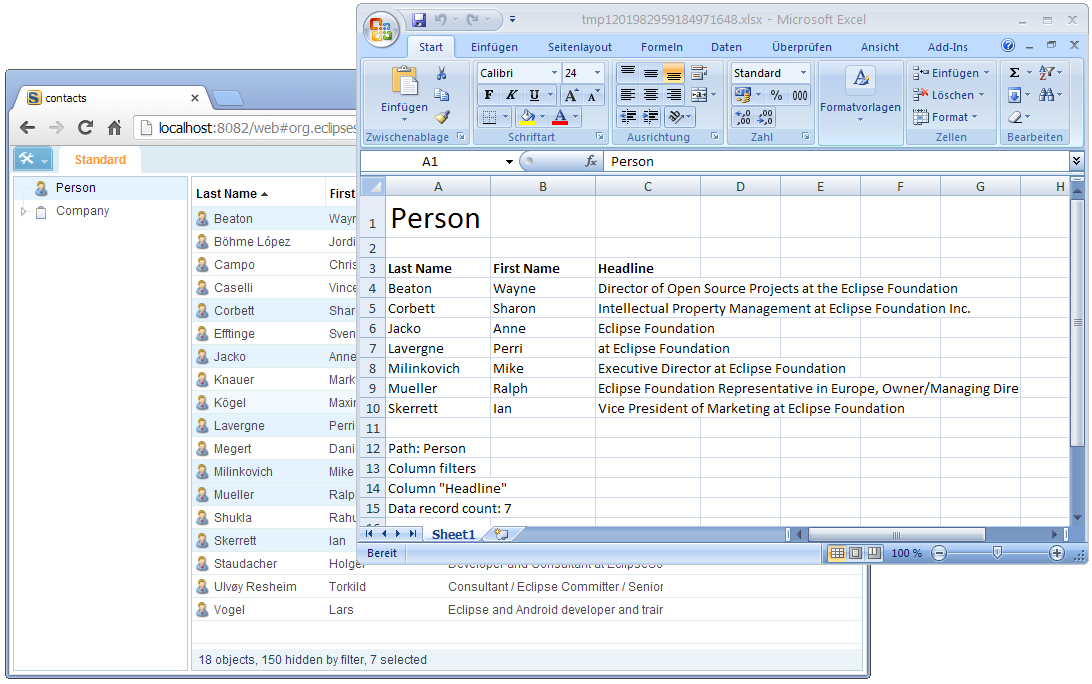
\includegraphics[width=14cm]{my_contacts_rapweb_excelexport.png} 
\caption{The ''My Contacts'' application running in the browser as web application. 
The Excel sheet shown in the front is exported from the person page using the 'Tools/Export to Excel' menu. }
\figlabel{my_contacts_rapweb_excelexport}
\end{figure}

\begin{figure}
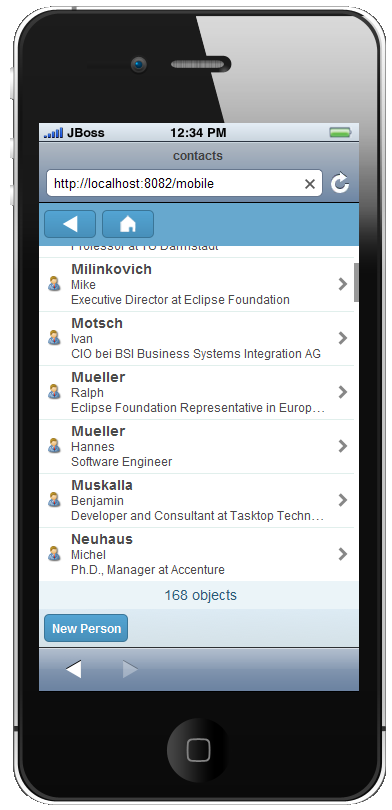
\includegraphics[width=6cm]{my_contacts_rapmobile_1.png} \hspace{5mm}
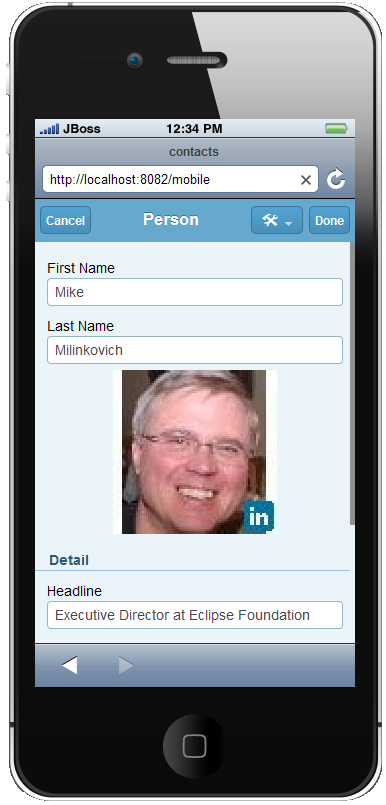
\includegraphics[width=6cm]{my_contacts_rapmobile_2.png} \hspace{5mm}
\caption{The ''My Contacts'' application running on an iPhone device. 
On the left hand side, the person page is shown. The person form is shown on the right. }
\figlabel{my_contacts_rapmobile}
\end{figure}

In \figref{my_contacts_rapweb_excelexport} the ''My Contacts'' application is running in a web browser. 
In this example, the \menu{Tools|Export to to Excel} is used to export the selectd row into an Excel sheet. 
Finally, the ''My Contacts'' application is also running on iPhone and Android mobile devices out of the box. 
Two example screens are provided in \figref{my_contacts_rapmobile}.

Once you no longer feel confident about having the ''My Contacts'' application accessing you data you can revoke this access permission in the LinkedIn menu ''Privacy and Settings''. 
In the lower part of the settings page switch to tab ''Groups, Companies and Applications'' and click on the link ''View your applications''. 
There, you will find again the partner name ''OAuth test for Scribe''. 
To revoke the access, select the associated checkbox and click the ''Remove'' button. 
The next time you try to referesh your LinkedIn data from the ''My Contacts'' application will result in an Error message. 
Before you can again access data from your LinkedIn accout you just need to refresh the access token as described above.

% --------------------------------------------------------------------------- %
\section{Setting up the new Scout project}

\begin{figure}
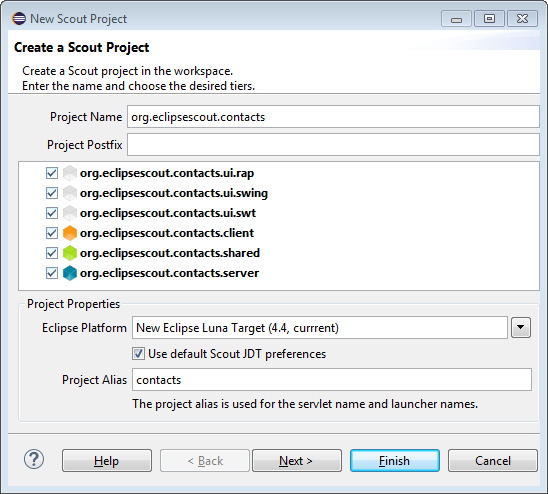
\includegraphics[width=7cm]{new_project_contacts_1.png} \hspace{5mm}
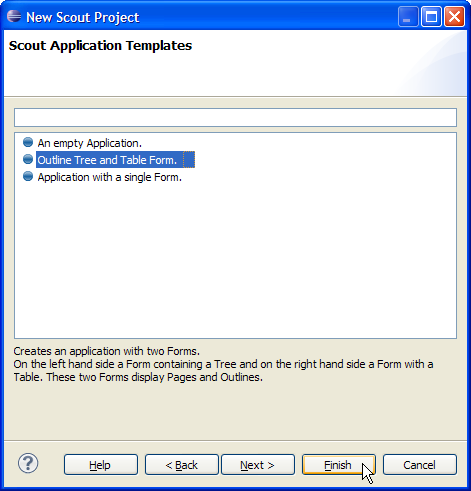
\includegraphics[width=7cm]{new_project_contacts_2.png}
\caption{Start with creating a new Scout project. }
\figlabel{new_project_contacts}
\end{figure}

The initial code for the ''My Contacts'' application is generated using the \wizard{New Scout Project} as decribed in \secref{wizard_new_project}. 
For the \field{Project Name} use the name \java{org.eclipsescout.contacts} as shown on the left side of \figref{new_project_contacts} and click on the \button{Next}. 
In the second wizard step select the application template \element{Outline Tree and Table Form} as shown on the right side of \figref{new_project_contacts}.

\begin{figure}
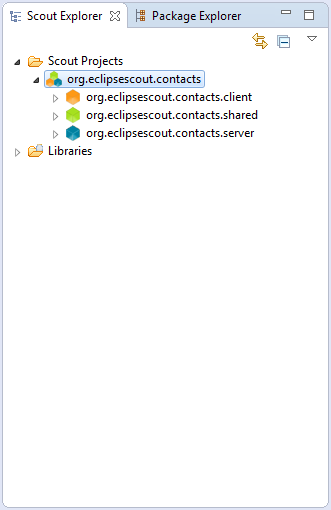
\includegraphics[width=7cm]{project_contacts_explorer.png} \hspace{5mm}
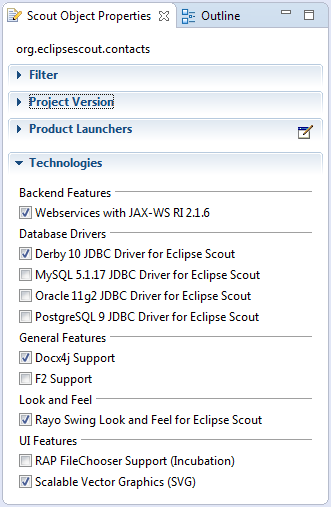
\includegraphics[width=7cm]{project_contacts_properties.png}
\caption{The setting of the \textit{Technology} section in the Scout Object Properties of the ''My Contacts'' application.}
\figlabel{project_contacts_properties}
\end{figure}

After the Scout SDK has created the initial application code select the top-level \node{org.eclipsescout.contacts} in the Scout Explorer. 
In the technology section of the corresponding Scout Object Properties select the Derby database driver, the Docx4j support and the Rayo look and feel as shown on the right side of \figref{project_contacts_properties}.
In case you have not yet selected either the Scout Docx4j support or the Rayo look and feel components, the Scout SDK will download these packages from the Eclipse Marketplace\footnote{
See \secref{scout_sdk_object_properties} for additional information regarding the download of marketplace packages}. 

\begin{figure}
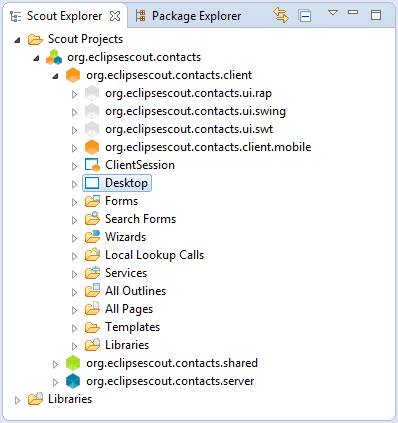
\includegraphics[width=7cm]{desktop_explorer.png} \hspace{5mm}
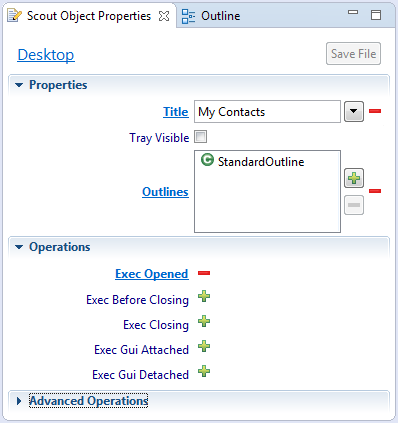
\includegraphics[width=7cm]{desktop_properties.png}
\caption{Configure the application name in the title field of the Desktop's properties. }
\figlabel{desktop_properties}
\end{figure}

To set the applications name select the \node{Desktop} in the Scout Explorer to access it's Scout Object Properties as shown in \figref{desktop_properties}.
In the \field{Title} enter the string ''My Contacts'' create a new translated text entry. 
Then click on the \link{Exec Opened} in the Scout Object Properties to access the Java code of this method. 

\lstinputlisting[
  label=\lstlabel{mycontacts.desktop.execopened},
  caption=The \java{execOpened} method of desktop class of the "My Contacts" application. The application's organisation into a tree and a table form is defined here.,
  index={execOpened,Desktop,UserAgentUtility},
  linerange={49-70},
  float
]
{../code/oneDayTutorial/org.eclipsescout.contacts.client/src/org/eclipsescout/contacts/client/ui/desktop/Desktop.java}

As shown in \lstref{mycontacts.desktop.execopened} the application's organisation into a tree and a table form is explicitly defined in method \java{execOpened}. 
First, using the \java{UserAgentUtility} class, the method checks if the client is working with a desktop or a web client. 
If not, the method returns and not tree and table setup is used. 
Instead, the \java{MobileHomeForm} defined in plugin \element{org.eclipsescout.contacts.client.mobile} is used. 
In case the user is working with a web client or a desktop client, default tree and table forms are created and started. 
Finally, the currently active outline is set to the \java{StandardOutline}, as this is the only outline defined in this application.

% --------------------------------------------------------------------------- %
\section{Adding the Person Page}

\begin{figure}
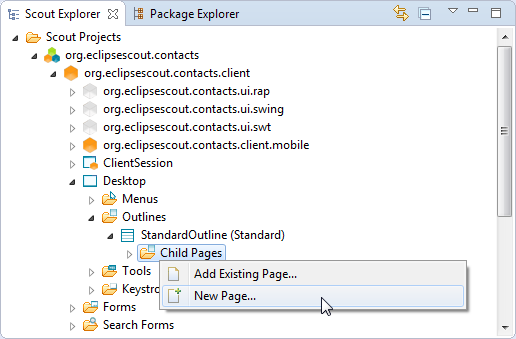
\includegraphics[width=5cm]{new_page_person_contextmenu.png} \hspace{2mm}
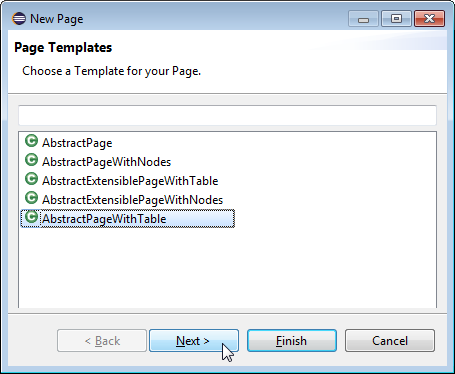
\includegraphics[width=4.5cm]{new_page_person_1.png} \hspace{2mm}
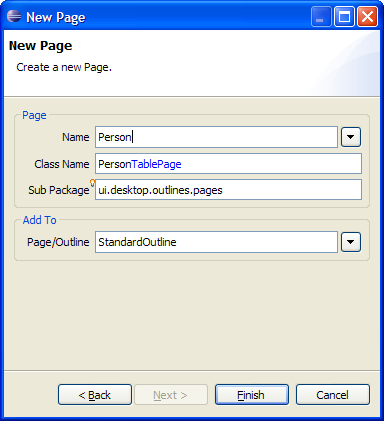
\includegraphics[width=4.5cm]{new_page_person_2.png}
\caption{Add the person table page below the standard outline. }
\figlabel{new_page_person}
\end{figure}

The first UI component we add to the application is the person page. 
For the desktop clients, this page is represented as a table that will list all available persons in the database of the ''My Contacts'' application. 
To start the \wizard{New Page} use the \contextmenu{New Page...} on the \folder{Child Pages} as shown in \figref{new_page_person}.
On the first wizard step select the template \element{AbstractPageWithTable} and click the \button{Next}. 
On the second wizard step, provide the page name ''Person'' to create a new translated text entry at the same time. 
Make sure the other fields are filled in as shown in \figref{new_page_person} and click the \button{Finish} to close the wizard.

\lstinputlisting[
  label=\lstlabel{mycontacts.desktop.outline.personpage},
  caption=The \java{execCreateChildPages} method of the standard outline. At the current implementation step the company table page is not (yet) added.,
  index={execCreateChildPages, StandardOutline},
  linerange={19-25},
  float
]
{../code/oneDayTutorial/org.eclipsescout.contacts.client/src/org/eclipsescout/contacts/client/ui/desktop/outlines/StandardOutline.java}

\lstref{mycontacts.desktop.outline.personpage} shows the created method \java{execCreateChildPages} that links the newly created person page to the standard outline. 
Note that your code will only look the same once you have added the company page in a later step of the implementation of this application.

\begin{figure}
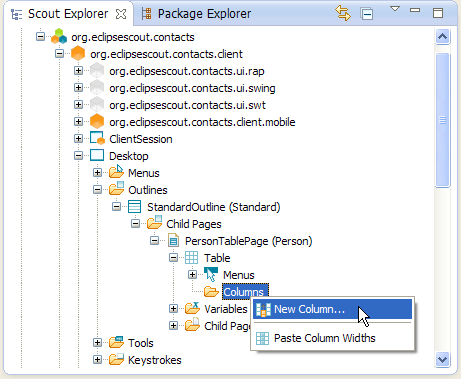
\includegraphics[width=5cm]{new_column_personid_contextmenu.png} \hspace{2mm}
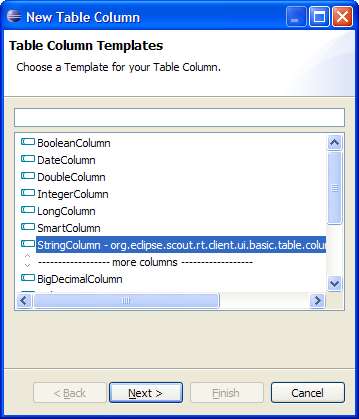
\includegraphics[width=4.5cm]{new_column_personid_1.png} \hspace{2mm}
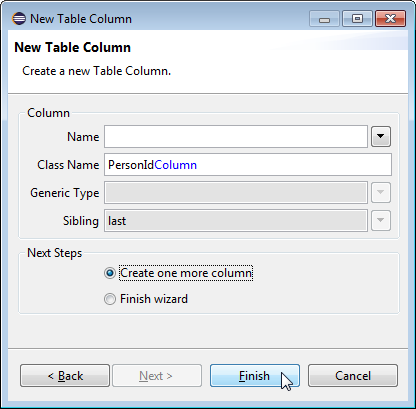
\includegraphics[width=4.5cm]{new_column_personid_2.png}
\caption{Add columns to the person page.}
\figlabel{new_column_personid}
\end{figure}

Now, drill down to the \folder{Columns} under the \node{PersonTablePage} as shown in \figref{new_column_personid}. 
Here we can add the desired table columns to the person page. 
Start with the column that will hold the person id. 
For this, start the column wizard as shown on the left side of \figref{new_column_personid} and select the string column template. 
In the second wizard step, enter ''PersonId'' into the \field{Class Name},select the radio button \element{Create one more column} and click on the \button{Finish}. 
This will restart the column wizard to enter the next columns. 
Create the remaining string columns with the following names.

\begin{itemize}
  \item{First Name}
  \item{Last Name}
  \item{Headline}
\end{itemize}

\begin{figure}
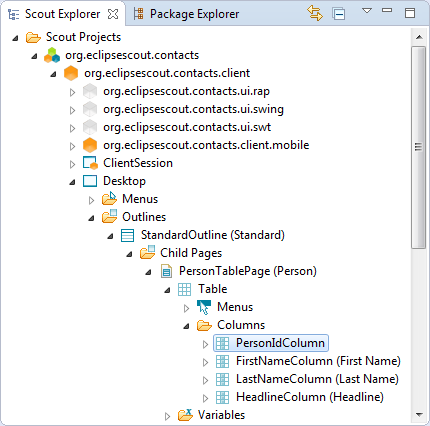
\includegraphics[height=7cm]{person_id_column.png} \hspace{5mm}
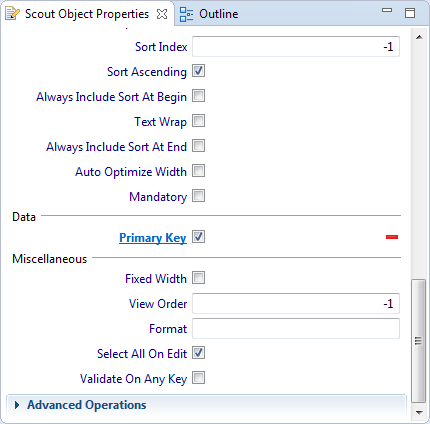
\includegraphics[height=7cm]{person_id_property.png}
\caption{Configure the \element{PersonId} column. Check property \element{Primary Key} under the section \element{Advanced Properties} (right).}
\figlabel{new_column_personid}
\end{figure}

\lstinputlisting[
  label=\lstlabel{mycontacts.desktop.outline.personpage.columns},
  caption=The person id and the first name columns of the \java{PersonTablePage} class. ,
  index={A primary key table column and a default string column.},
  linerange={71-93},
  float
]
{../code/oneDayTutorial/org.eclipsescout.contacts.client/src/org/eclipsescout/contacts/client/ui/desktop/outlines/pages/PersonTablePage.java}

Once you have created all these columns we will mark the person id column as the primary key column for the person page. 
In the Scout Explorer select the \node{PersonIdColumn} to open the corresponding Scout Object Properties. 
In this form, deselect the \property{Displayable} to always hide this technical column from the end user. 
In the properties \element{Advanced Properties} section check the \property{Primary Key}. 
The resulting Java code for the primary key column and the first name column is provided in \lstref{mycontacts.desktop.outline.personpage.columns}. 

\begin{figure}
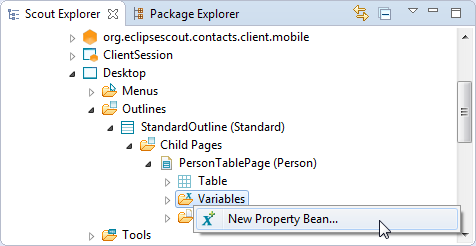
\includegraphics[height=5cm]{new_bean_companyid_contextmenu.png} \hspace{5mm}
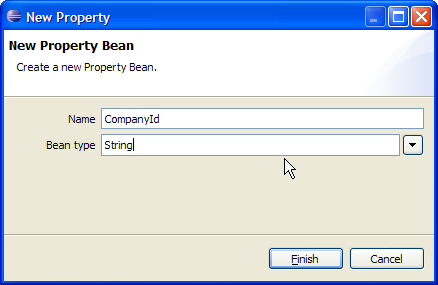
\includegraphics[height=5cm]{new_bean_companyid.png}
\caption{Add the \element{CompanyId} variable to the person page.}
\figlabel{new_bean_companyid}
\end{figure}

\lstinputlisting[
  label=\lstlabel{mycontacts.desktop.outline.personpage.columns},
  caption=The company id variable of the \java{PersonTablePage} class. ,
  index={A table page property bean.},
  linerange={18-21,162-172},
  float
]
{../code/oneDayTutorial/org.eclipsescout.contacts.client/src/org/eclipsescout/contacts/client/ui/desktop/outlines/pages/PersonTablePage.java}

As we will later add and link the person page with a company page, we add a company id variable to the person page as shown in \figref{new_bean_companyid}. 
For the Java representation of such variables the standard bean pattern is used as shown in \lstref{mycontacts.desktop.outline.personpage.columns}.

% --------------------------------------------------------------------------- %
\section{Adding the Company Page}

\begin{figure}
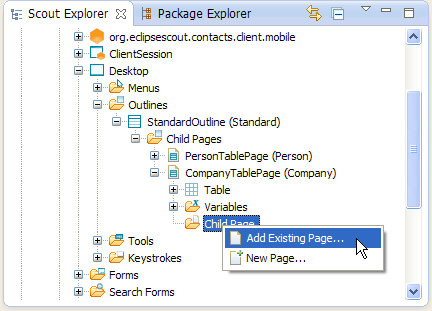
\includegraphics[width=6.5cm]{add_existing_page_contextmenu.png} \hspace{5mm}
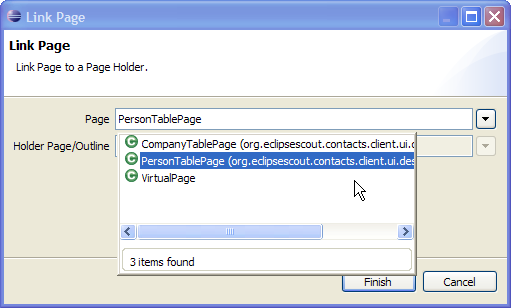
\includegraphics[width=7.5cm]{add_existing_page.png}
\caption{Add the person page below the the company page.}
\figlabel{add_existing_page}
\end{figure}

\lstinputlisting[
  label=\lstlabel{mycontacts.desktop.outline.companypage.linking},
  caption=Linking the \java{PersonTablePage} with the parent \java{CompanyTablePage}.,
  index={Linking pages hierachically.},
  linerange={30-36},
  float
]
{../code/oneDayTutorial/org.eclipsescout.contacts.client/src/org/eclipsescout/contacts/client/ui/desktop/outlines/pages/CompanyTablePage.java}

After adding the person page, we add a company page to the standard outline. 
To add the company page we use the same wizards as described in the previous section for the person page. 
For the \field{Name} we enter the new translated text ''Company'' and the columns to add are the following.

\begin{itemize}
  \item{Company Id}
  \item{Name}
  \item{Location}
\end{itemize}

As in the case of the person table page, the company id column is used as a primary key column. 
The \property{Displayable} needs to be set to false and the \property{Primary Key} to true. 
Now we can link the person page to the company page using the \contextmenu{Add Existing Page...} as shown on the left side of \figref{add_existing_page}. 
In the \wizard{Link Page}, the person page can then be selected according to the right side of \figref{add_existing_page}. 
In the Java code generated by the Scout SDK the setting of the company id attribute is automatically inserted in method \java{execCreateChildPage}. 
Please note that this convenience added by the Scout SDK wizard only works if the child page defines variables with a naming that matches the defined primary key columns of the parent table. 

% --------------------------------------------------------------------------- %
\section{Installing the Database}

\begin{figure}
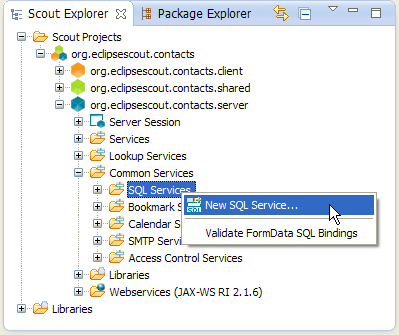
\includegraphics[width=7cm]{new_service_derby_contextmenu.png} \hspace{5mm}
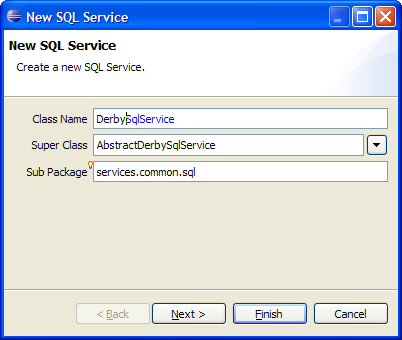
\includegraphics[width=7cm]{new_service_derby.png} 
\caption{Add the service to access the Derby database under folder \element{SQL Services}. }
\figlabel{new_service_derby}
\end{figure}

To access a database we first need to install a database service. 
For the ''My Contacts'' application, this is done using the \wizard{New SQL Service} on the Scout server under the \folder{SQL Services} as shown in \figref{new_service_derby}.
In the first wizard step shown on the right side of the figure, use ''DerbySqlService'' for the \field{Class Name}.
From the drop-down list in the \field{Super Class} choose the \java{AbstractDerbySqlService} and click on the \button{Finish}.

\lstinputlisting[
  label=\lstlabel{mycontacts.server.configini.derby},
  caption=Setting up the database parameters in the Scout server's \texttt{config.ini} file.,
  index={database setup, config.ini},
  linerange={42-48},
  float
]
{../code/oneDayTutorial/org.eclipsescout.contacts.server/products/development/config.ini}

To setup the database connection the necessary parameters need to be added to the server's \filename{config.ini} file as shown in \lstref{mycontacts.server.configini.derby}.
Comparing the parameter names in this config file with the package name of the created \java{DerbySqlService} service class reveals an interesting framework feature. 
All Scout services can be parameterized using the \filename{config.ini} file with the pattern \java{<package>.<class name>\#<parameter>=<value>}. 
The Scout runtime then sets the service parameters using matching setter methods such as \java{setPassword} for the password parameter.  

According to the parameter \java{jdbcMappingName=jdbc:derby:\$\{workspace\_loc\}/...} a new Derby database will be created in the same parent directory as the ''My Contacts'' workspace directory if no database named \java{DB\_CONTACT} is found there.
This setup is handy for development purposes but you may want to set the database parameter to \java{create=false} in the \filename{config.ini} of the production product file. 

\begin{figure}
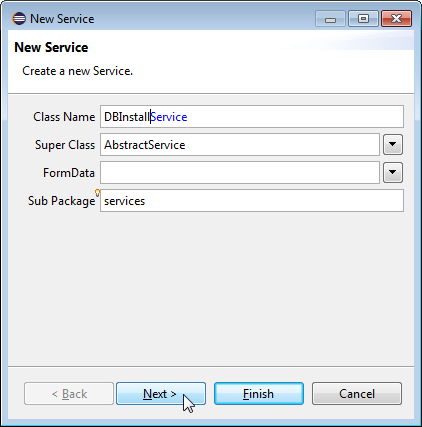
\includegraphics[width=7cm]{new_service_dbinstall_1.png} \hspace{5mm}
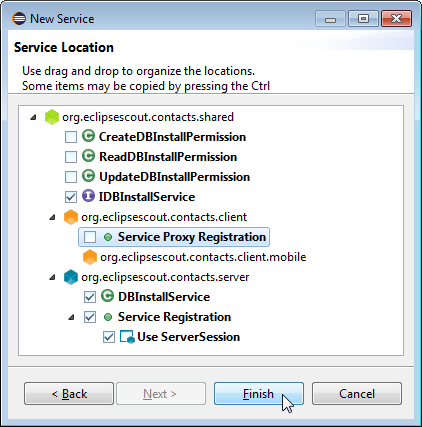
\includegraphics[width=7cm]{new_service_dbinstall_2.png} 
\caption{Add a database installation service. }
\figlabel{new_service_dbinstall}
\end{figure}

\begin{figure}
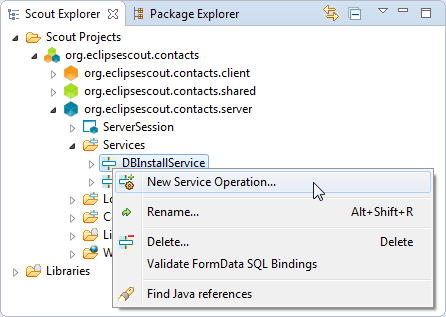
\includegraphics[height=5.5cm]{new_operation_installstorage_contextmenu.png} \hspace{5mm}
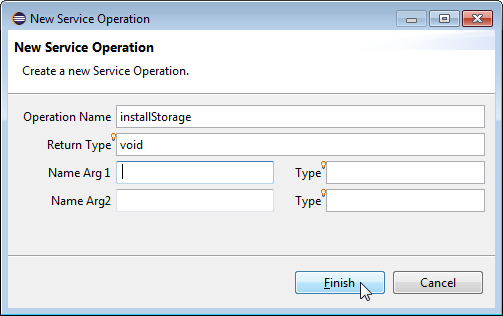
\includegraphics[height=5.5cm]{new_operation_installstorage.png} 
\caption{Add the service operation to create the DB schema. }
\figlabel{new_operation_installstorage}
\end{figure}


\lstinputlisting[
  label=\lstlabel{mycontacts.server.services.installdb},
  caption=The \java{installStorage} service operation to create the database schema for the ''My Contacts'' application.
  New tables are created if they are not found by \java{getExistingTables} in the existing schema.,
  index={A service operation to install a database schema.},
  linerange={14-15,26-36,94-105},
  float
]
{../code/oneDayTutorial/org.eclipsescout.contacts.server/src/org/eclipsescout/contacts/server/services/DBInstallService.java}

% ........................................................................... %
\subsection{Setting up the Database Schema}

Having a working database service and a new (empty) Derby database now allows to create the necessary database schema and populate it with some initial data.
For this we add a new \java{DBInstallService} service as shown in \figref{new_service_dbinstall}.
To this install service we then add the \java{installStorage} operation according to \figref{new_operation_installstorage}.
The implementation of this method is provided in \lstref{mycontacts.server.services.installdb}.
The method first checks if a setup is requried. 
For this, the member variable \java{m\_doSetup} is used that might also be set by the \java{setDoSetup} setter method via the server's the \filename{config.ini} file.

\lstinputlisting[
  label=\lstlabel{mycontacts.server.services.installdb.company},
  caption=Setting up the \java{COMPANY} table of the ''My Contacts'' application.,
  linerange={37-56},
  float
]
{../code/oneDayTutorial/org.eclipsescout.contacts.server/src/org/eclipsescout/contacts/server/services/DBInstallService.java}

\lstinputlisting[
  label=\lstlabel{mycontacts.server.services.installdb.person},
  caption=Setting up the \java{PERSON} table of the ''My Contacts'' application.,
  linerange={57-79},
  float
]
{../code/oneDayTutorial/org.eclipsescout.contacts.server/src/org/eclipsescout/contacts/server/services/DBInstallService.java}

\lstinputlisting[
  label=\lstlabel{mycontacts.server.services.installdb.users_param},
  caption=Setting up the \java{USERS\_PARAM} table of the ''My Contacts'' application.,
  linerange={80-94},
  float
]
{../code/oneDayTutorial/org.eclipsescout.contacts.server/src/org/eclipsescout/contacts/server/services/DBInstallService.java}

Setting up the schema to contain the indiviudal tables for the ''My Contacts'' application is implemented in a separate method per table. 
The table definition for the company table is provided in \lstref{mycontacts.server.services.installdb.company}. 
In this method two Scout aspects are of interest. 

The first Scout feature used is the absence of a \java{COMMIT} statement after the two \java{INSERT INTO} statements. 
This is possible, as all Scout service calls run in a transaction context that is transparent to the Scout developer. 
If a service method exits without errors, the enclosing transaction is committed. 
And if any runtime exception occurs in a service call the Scout runtime framework performs a rollback.

The second feature is the parameter binding used in the \java{INSERT INTO} statements. 
When SQL statements are executed using any of the static \java{SQL} methods, an internal statement processor replaces all bind variables found in the provided statement string. 
In Scout, SQL bind variables need to use the pattern \java{:<variable name>}. 
The values for the bind variables can then be provided in the form of additional arguments. 
In the concrete example of \lstref{mycontacts.server.services.installdb.company}, the content for the bind variable \java{:company\_id} is provided as a \java{NVPair} object. 
\element{NVPairs} are the simplest possible form to represent bind variables. 
The first constructor argument is the variable name of the bind variable, in this case \java{company\_id}. 
The actual content of the bind variable is provided in the form of an object. 
Here, the Java runtime class \java{UUID.randomUUID().toString()} is used to create a new company key. 

Setting up the person table and the user parameter table is defined according to \lstref{mycontacts.server.services.installdb.person} and \lstref{mycontacts.server.services.installdb.users_param}. 
To create a data object for the persons day of birth, the Scout utility class \java{DateUtility} is used.

\lstinputlisting[
  label=\lstlabel{mycontacts.server.serverapplication},
  caption=Scheduling the database installation in the \java{start} method of the \java{ServerApplication} class during the server application startup.,
  index={ServerApplication, ServerSession},
  linerange={30-57,62-63},
  float
]
{../code/oneDayTutorial/org.eclipsescout.contacts.server/src/org/eclipsescout/contacts/server/ServerApplication.java}

The only piece missing to setup the database is calling the \java{installStorage} operation during the startup of the ''My Contacts'' server application.
The proper way to implement such a scenario is to schedule an installation job in the \java{ServerApplication} class of the Scout server. 
In the ''My Contacts'' application this is implemented according to \lstref{mycontacts.server.serverapplication}. 
To create a server job, a new server session object needs to be obtained first. 
However, during the startup time of the server we do not have any logged in users yet. 
That is why the session is created for the backend subject representing the server application. 
Using this \java{serverSession} object, the \java{installJob} can be created. 
In it's \java{runTransaction} method we can then call the \java{installStorage} operation to setup the ''My Contacts'' database.

% ........................................................................... %
\subsection{Scout Logging}

\lstinputlisting[
  label=\lstlabel{mycontacts.server.configini.logging},
  caption=The logging configuration in the Scout server's \texttt{config.ini} file.,
  index={config.ini, logging setup},
  linerange={14-17},
  float
]
{../code/oneDayTutorial/org.eclipsescout.contacts.server/products/development/config.ini}

An additional Scout topic that is touched in this \java{ServerApplication} class is the Scout logging. 
As shown in \lstref{mycontacts.server.serverapplication}, a static \java{logger} object is created using Scout's \java{ScoutLogManager} class. 
Events can then be logged with the \java{logger.info} method where \java{info} refers to the log level attached to this message. 
Similar to the database setup described above, the logging setup can be defined in \filename{config.ini} file. 
The default setup defined for the development product is provided in \lstref{mycontacts.server.configini.logging}.
Further information regarding logging in Eclipse Scout is available in the Scout wiki\footnote{
Logging in Eclipse Scout: \url{http://wiki.eclipse.org/Scout/Concepts/Logging}.
}.

% --------------------------------------------------------------------------- %
\section{Fetching Data from the Database}

\begin{figure}
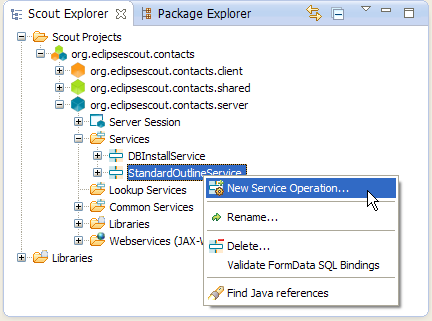
\includegraphics[height=5cm]{new_service_persontabledata_contextmenu.png} \hspace{5mm}
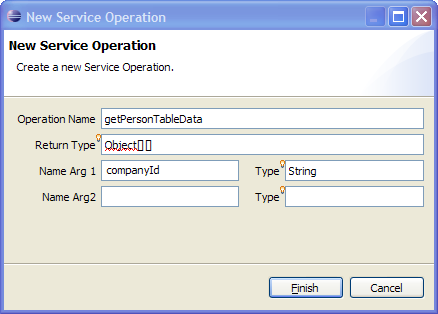
\includegraphics[height=5cm]{new_service_persontabledata.png}
\caption{Add the service operation to fetch the data for the person table. }
\figlabel{new_service_persontabledata}
\end{figure}

In the section before, we have implemented the access to the Derby database for the Scout server. 
And during the server startup, the application's database schema can now be created and populated with some initial data. 

Here, this schema and the implemented database access is used to fetch the data for the client application's person page and the company page. 
The best place to implement these data provider methods is in the server's \java{StandardOutlineService} class. 
This class has been created by the Scout SDK during the initial project creation step.
It is meant to hold the operations that fetch the data for populating the elements visible in the outline tree and outline pages. 

For the ''My Contacts'' application, we first create the \java{getPersonTableData} operation as shown in \figref{new_service_persontabledata}. 
In the wizard dialog enter ''getPersonTableData'' into the \field{Operation Name}. 
For the return type we simply use a two dimensional object array. 
As the person page is also displayed under the company page, we need to have a way to only return the persons working for a specific company. 
To allow for this use case, we add the parameter ''companyId'' as the first argument to the \java{getPersonTableData} operation before we close the wizard with \button{Finish}. 

The next operation we need is the \java{getCompanyTableData} method. 
You may use the same creation steps as described above for the person table page data. 
But for fetching company table data we do not need an additional argument.
The company page in the ''My Contacts'' application will always show all available companies. 

\lstinputlisting[
  label=\lstlabel{mycontacts.server.services.standardoutline},
  caption=Fetching the table data for the person and the company page of the ''My Contacts'' application.
  The list of persons is restricted to employees of a specific company if a company id parameter is provided.,
  index={SQL, StringUtility, bind variables, NVPair, StandardOutlineService},
  linerange={10-29},
  float
]
{../code/oneDayTutorial/org.eclipsescout.contacts.server/src/org/eclipsescout/contacts/server/services/StandardOutlineService.java}

For the actual implementation of the two data fetching operations the code provided in \lstref{mycontacts.server.services.standardoutline} is used. 
The implementation is straight forward and almost trivial. 
However, we can use the \java{getPersonTableData} example to introduce one of the many Scout utility classes. 

\begin{figure}
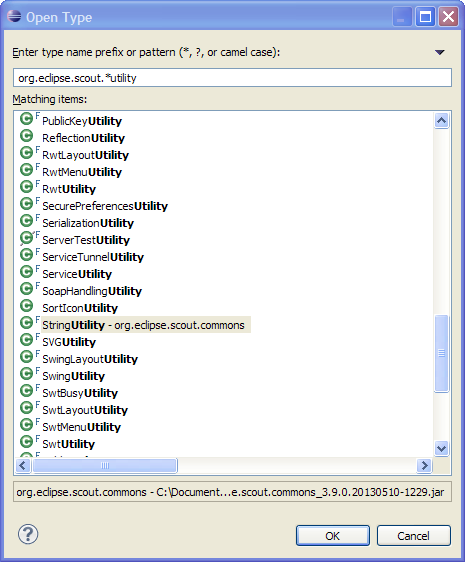
\includegraphics[width=8cm]{scout_utility_classes.png}
\caption{Accessing the Scout utility classes with the pattern \java{org.eclipse.scout.*Utility}.}
\figlabel{scout_utility_classes}
\end{figure}

The class \java{StringUtility} is one of the many utility classes provided by the Scout framework. 
Here, it is used for the typical null or empty check. 
To get a quick overview, hit the \key{Ctrl}\key{Shift}\key{T} key combination. 
In the type dialog that appears enter \java{org.eclipse.scout.*Utility} into the pattern field. 
This will display the complete list of the Scout utility classes as shown in \figref{scout_utility_classes}.

% --------------------------------------------------------------------------- %
\section{Creating the Person Form}

\begin{figure}
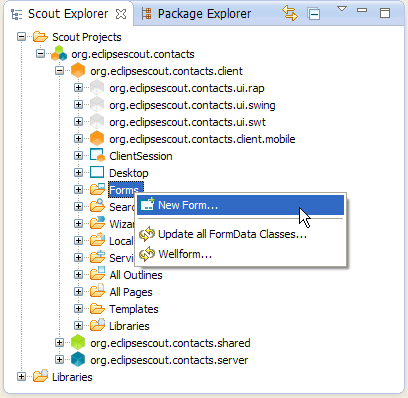
\includegraphics[height=7cm]{new_form_person_contextmenu.png} \hspace{5mm}
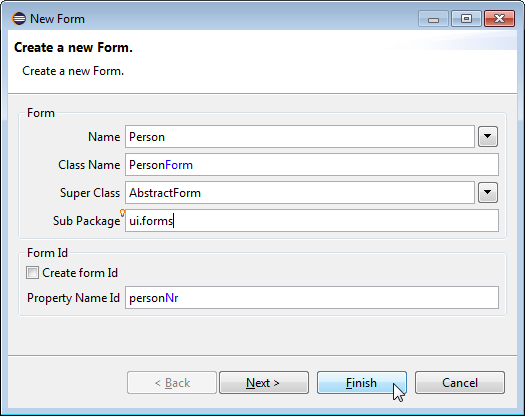
\includegraphics[height=7cm]{new_form_person.png}
\caption{Add the person form.}
\figlabel{new_form_person}
\end{figure}

In this section we will create the person form that is used to display and edit the persons stored in the ''My Contacts'' application. 
To add the person form use the Scout SDK \wizard{New Form} as shown in \figref{new_form_person}. 
In the first wizard step you just need to enter ''Person'' as a new translated text into the \field{Name} and add ''ui.forms'' as the sub-package name in the corresponding wizard field. 
Then click the \button{Finish}.

The wizard will create the necssary artefacts in the application's client, the shared and the server plugin projects. 
On the client side the \java{PersonForm} class with the necessary form handlers is created, in the shared part, the \java{PersonFormData} transfer object is added. 
On the server side, a \java{PersonProcessService} with all necessary service operations referenced by the form handlers is implemented. 

\begin{figure}
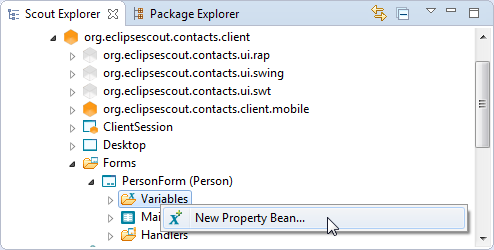
\includegraphics[height=4.5cm]{new_bean_personid_contextmenu.png} \hspace{5mm}
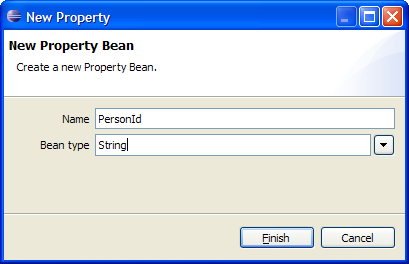
\includegraphics[height=4.5cm]{new_bean_personid.png}
\caption{Add the \element{PersonId} variable to the person form.}
\figlabel{new_bean_personid}
\end{figure}

To hold the persons primary key in the person form we also need to add a corresponding variable. 
For this, use the \wizard{New Property Bean} as shown in \figref{new_bean_personid}. 
In the wizard dialog, enter ''PersonId'' into the \field{Name} and pick \java{String} from the dropdown list provided in the \field{Bean type}. 
Then, click the \button{Finish} to close the wizard. 

\begin{figure}
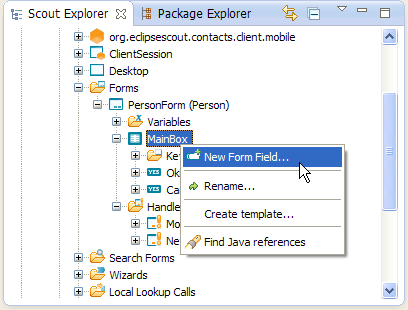
\includegraphics[width=7cm]{new_field_personbox.png} \hspace{5mm}
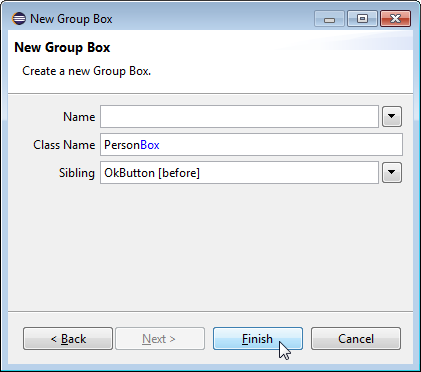
\includegraphics[width=7cm]{new_field_personbox_name.png}
\caption{Add the first group box field to the person form.}
\figlabel{new_field_personbox}
\end{figure}

Lorem ipsum will build an outline based Scout application featuring a navigation tree and pages to present information in tabular form. 
In addition, the application also shows how to work with menus and context menus, search forms, and forms to enter and/or update data. 
On the server side we show how to work with databases, how to use logging in Scout applications and how to lorem ipsum. 

\begin{figure}
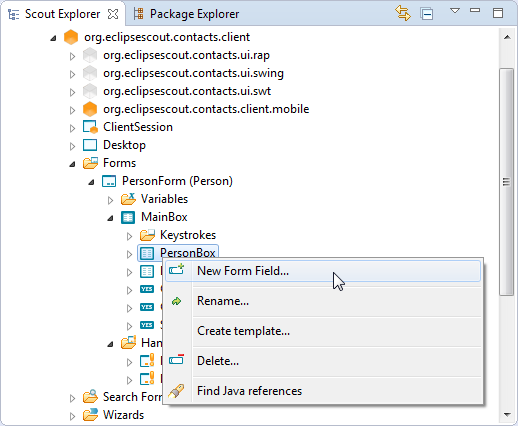
\includegraphics[width=7cm]{new_field_picture_contextmenu.png} \hspace{5mm}
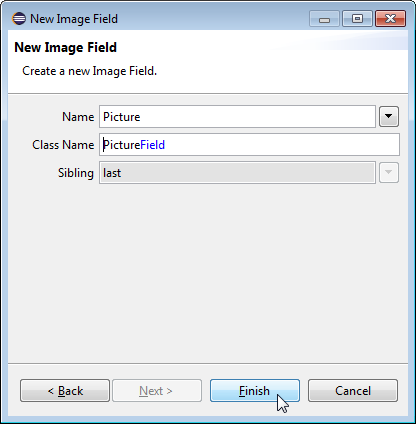
\includegraphics[width=7cm]{new_field_picture.png}
\caption{Add the picture field to the first group box of the person form.}
\figlabel{new_field_picture}
\end{figure}

\lstinputlisting[
  label=\lstlabel{mycontacts.client.forms.person.picturefield},
  caption=The behaviour of the person form's \java{PictureField} is triggered by changes in field \java{PictureUrlField}.,
  index={getConfiguredMasterField, execChangedMasterValue, IOUtility},
  linerange={133-135,151-167,186-187},
  float
]
{../code/oneDayTutorial/org.eclipsescout.contacts.client/src/org/eclipsescout/contacts/client/ui/forms/PersonForm.java}

Lorem ipsum will build an outline based Scout application featuring a navigation tree and pages to present information in tabular form. 
In addition, the application also shows how to work with menus and context menus, search forms, and forms to enter and/or update data. 
On the server side we show how to work with databases, how to use logging in Scout applications and how to lorem ipsum. 

\begin{figure}
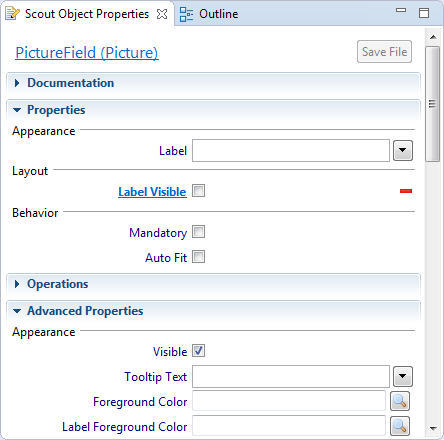
\includegraphics[width=7cm]{picture_field_properties_1.png} \hspace{5mm}
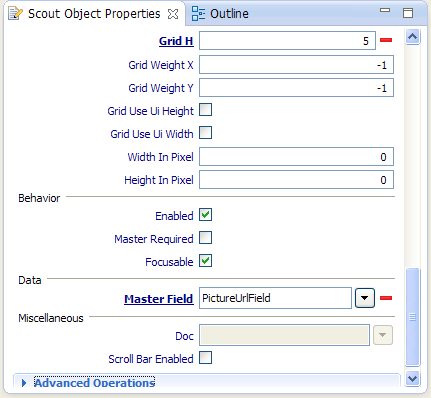
\includegraphics[width=7cm]{picture_field_properties_2.png}
\caption{Set the properties for the picture field of the person form.}
\figlabel{picture_field_properties}
\end{figure}

\lstinputlisting[
  label=\lstlabel{mycontacts.client.forms.person.picturefield.properties},
  caption=The Java code for the selected Scout Object Properties of the \java{PictureField}.,
  index={getConfiguredMasterField, execChangedMasterValue, IOUtility},
  linerange={133-150,186-187},
  float
]
{../code/oneDayTutorial/org.eclipsescout.contacts.client/src/org/eclipsescout/contacts/client/ui/forms/PersonForm.java}

Lorem ipsum will build an outline based Scout application featuring a navigation tree and pages to present information in tabular form. 
In addition, the application also shows how to work with menus and context menus, search forms, and forms to enter and/or update data. 
On the server side we show how to work with databases, how to use logging in Scout applications and how to lorem ipsum. 

\begin{figure}
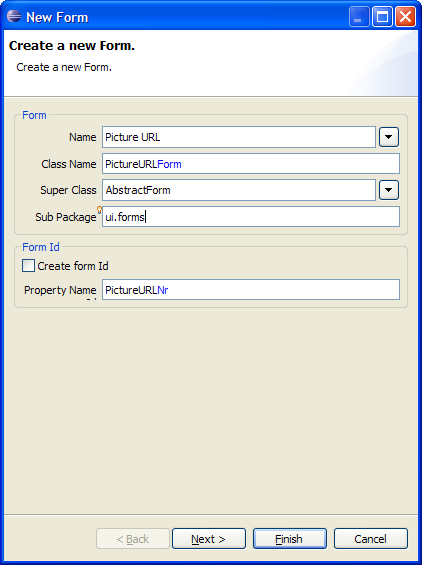
\includegraphics[width=7cm]{new_form_url_1.png} \hspace{5mm}
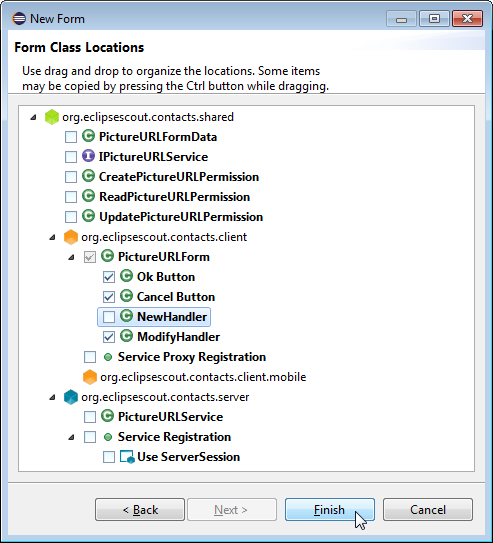
\includegraphics[width=7cm]{new_form_url_2.png}
\caption{Add the URL editor form.}
\figlabel{new_form_url}
\end{figure}

\lstinputlisting[
  label=\lstlabel{mycontacts.client.forms.pictureurl},
  caption=The UI structure of the \java{PictureURLForm} used to update the URL of the picture field in the person form.,
  linerange={17-18,52-67,79-80},
  float
]
{../code/oneDayTutorial/org.eclipsescout.contacts.client/src/org/eclipsescout/contacts/client/ui/forms/PictureURLForm.java}

Lorem ipsum will build an outline based Scout application featuring a navigation tree and pages to present information in tabular form. 
In addition, the application also shows how to work with menus and context menus, search forms, and forms to enter and/or update data. 
On the server side we show how to work with databases, how to use logging in Scout applications and how to lorem ipsum. 

\begin{figure}
\includegraphics[width=7cm]{new_menu_editurl_contextmenu.png} \hspace{5mm}
\includegraphics[width=7cm]{new_menu_editurl.png}
\caption{Add the URL edit menu to the picture field.}
\figlabel{new_menu_editurl}
\end{figure}

\lstinputlisting[
  label=\lstlabel{mycontacts.client.forms.person.picturefield.editmenu},
  caption=The edit menu implemented in class \java{EditURLMenu} of the picture field.
  If the URL was changed the picture URL field of the person form is set accordingly in method \java{execAction},
  index={execAction},
  linerange={168-185},
  float
]
{../code/oneDayTutorial/org.eclipsescout.contacts.client/src/org/eclipsescout/contacts/client/ui/forms/PersonForm.java}

Lorem ipsum will build an outline based Scout application featuring a navigation tree and pages to present information in tabular form. 
In addition, the application also shows how to work with menus and context menus, search forms, and forms to enter and/or update data. 
On the server side we show how to work with databases, how to use logging in Scout applications and how to lorem ipsum. 

% --------------------------------------------------------------------------- %
\section{Integrating the Person Form into the Application}

\begin{figure}
\includegraphics[width=7cm]{new_menu_editperson_contextmenu.png} \hspace{5mm}
\includegraphics[width=7cm]{new_menu_editperson.png}
\caption{Add the Person edit menu to the person page.}
\figlabel{new_menu_editperson}
\end{figure}

\lstinputlisting[
  label=\lstlabel{mycontacts.desktop.outline.personpage.editmenu},
  caption=The \java{EditPersonMenu} to edit the person selected in the person table.
  The person id taken from the corresponding (invisible) column is transferred to the person form before the form is started.,
  index={isFormStored, reloadPage},
  linerange={112-131},
  float
]
{../code/oneDayTutorial/org.eclipsescout.contacts.client/src/org/eclipsescout/contacts/client/ui/desktop/outlines/pages/PersonTablePage.java}

Lorem ipsum will build an outline based Scout application featuring a navigation tree and pages to present information in tabular form. 
In addition, the application also shows how to work with menus and context menus, search forms, and forms to enter and/or update data. 
On the server side we show how to work with databases, how to use logging in Scout applications and how to lorem ipsum. 

\begin{figure}
\includegraphics[height=5cm]{person_table_explorer.png} \hspace{5mm}
\includegraphics[height=5cm]{person_table_properties.png}
\caption{Set the behaviour for the row level action on the person table.}
\figlabel{person_table_properties}
\end{figure}

\lstinputlisting[
  label=\lstlabel{mycontacts.desktop.outline.personpage.execrowaction},
  caption=The \java{execRowAction} method on table pages is used to trigger an action when a row is selcted with a double click or \textsc{<Enter>}.,
  index={execRowAction},
  linerange={58-62},
  float
]
{../code/oneDayTutorial/org.eclipsescout.contacts.client/src/org/eclipsescout/contacts/client/ui/desktop/outlines/pages/PersonTablePage.java}

Lorem ipsum will build an outline based Scout application featuring a navigation tree and pages to present information in tabular form. 
In addition, the application also shows how to work with menus and context menus, search forms, and forms to enter and/or update data. 
On the server side we show how to work with databases, how to use logging in Scout applications and how to lorem ipsum. 

% --------------------------------------------------------------------------- %
\section{Extending the Person Form with a Company Smartfield}

\begin{figure}
\includegraphics[width=6cm]{new_lookupcall_company_contextmenu.png}
\caption{Add a lookup call to the applications shared node.}
\figlabel{new_lookupcall_company_contextmenu}
\end{figure}

\begin{figure}
\includegraphics[height=5.5cm]{new_lookupcall_company_1.png} \hspace{5mm}
\includegraphics[height=5.5cm]{new_lookupcall_company_2.png}
\caption{The two wizard steps to enter the details of the company lookup call.}
\figlabel{new_lookupcall_company}
\end{figure}

\lstinputlisting[
  label=\lstlabel{mycontacts.shared.lookup.companylookupcall},
  caption=The company lookup call with its \java{getConfiguredService} method in the application's shared plugin.,
  index={LookupCall, getConfiguredService},
  linerange={7-16},
  float
]
{../code/oneDayTutorial/org.eclipsescout.contacts.shared/src/org/eclipsescout/contacts/shared/services/lookup/CompanyLookupCall.java}

\lstinputlisting[
  label=\lstlabel{mycontacts.server.lookup.companylookupservice},
  caption=The company lookup service in the application's server plugin.
  The \java{key} and the \java{text} criterias are used to search for values by key or by the provided name substring.
  index={AbstractSqlLookupService, getConfiguredSqlSelect},
  linerange={6-20},
  float
]
{../code/oneDayTutorial/org.eclipsescout.contacts.server/src/org/eclipsescout/contacts/server/services/lookup/CompanyLookupService.java}

Lorem ipsum will build an outline based Scout application featuring a navigation tree and pages to present information in tabular form. 
In addition, the application also shows how to work with menus and context menus, search forms, and forms to enter and/or update data. 
On the server side we show how to work with databases, how to use logging in Scout applications and how to lorem ipsum. 

\begin{figure}
\includegraphics[width=7cm]{new_smartfield_company_contextmenu.png}
\caption{Add a smartfield to the person form.}
\figlabel{new_smartfield_company_contextmenu}
\end{figure}

\begin{figure}
\includegraphics[height=5cm]{new_smartfield_company_1.png} \hspace{5mm}
\includegraphics[height=5cm]{new_smartfield_company_2.png}
\caption{Create the company smartfield for the person form.}
\figlabel{new_smartfield_company}
\end{figure}

\lstinputlisting[
  label=\lstlabel{mycontacts.client.forms.person.companyfield},
  caption=The smartfield \java{CompanyField} of the person form and its wiring with the company lookup call.,
  index={AbstractSmartField, getConfiguredLookupCall},
  linerange={233-247},
  float
]
{../code/oneDayTutorial/org.eclipsescout.contacts.client/src/org/eclipsescout/contacts/client/ui/forms/PersonForm.java}

Lorem ipsum will build an outline based Scout application featuring a navigation tree and pages to present information in tabular form. 
In addition, the application also shows how to work with menus and context menus, search forms, and forms to enter and/or update data. 
On the server side we show how to work with databases, how to use logging in Scout applications and how to lorem ipsum. 


% --------------------------------------------------------------------------- %
\section{Adding the Scribe Library to the Application}

\begin{figure}
\includegraphics[width=7cm]{new_library_scribe_contextmenu.png} \hspace{5mm}
\caption{Add a new bundle to hold the Scribe JARs.}
\figlabel{new_library_scribe_contextmenu}
\end{figure}

Lorem ipsum will build an outline based Scout application featuring a navigation tree and pages to present information in tabular form. 
In addition, the application also shows how to work with menus and context menus, search forms, and forms to enter and/or update data. 
On the server side we show how to work with databases, how to use logging in Scout applications and how to lorem ipsum. 

\begin{figure}
\includegraphics[width=7cm]{new_library_scribe_1.png} \hspace{5mm}
\includegraphics[width=7cm]{new_library_scribe_2.png}
\caption{Specify the JARs to be contained in the library bundle and the library name.}
\figlabel{new_library_scribe}
\end{figure}

Lorem ipsum will build an outline based Scout application featuring a navigation tree and pages to present information in tabular form. 
In addition, the application also shows how to work with menus and context menus, search forms, and forms to enter and/or update data. 
On the server side we show how to work with databases, how to use logging in Scout applications and how to lorem ipsum. 

% --------------------------------------------------------------------------- %
\section{Integrating LinkedIn Access with Scribe}

\begin{figure}
\includegraphics[height=5.5cm]{new_operation_authurl_contextmenu.png} \hspace{5mm}
\includegraphics[height=5.5cm]{new_operation_authurl.png}
\caption{Add the operation to retrieve an authentication URL.}
\figlabel{new_operation_authurl}
\end{figure}

\lstinputlisting[
  label=\lstlabel{mycontacts.server.linkedin.initialize},
  caption=The \java{LinkedInService} service with it's \java{initializeService} method defined in the \java{IService} interface.,
  index={IService, initializeService},
  linerange={32-50,160-161},
  float
]
{../code/oneDayTutorial/org.eclipsescout.contacts.server/src/org/eclipsescout/contacts/server/services/LinkedInService.java}

\lstinputlisting[
  label=\lstlabel{mycontacts.server.linkedin.authurl},
  caption=The \java{getAuthUrl} method of the LinkedIn service.,
  index={AbstractSmartField, getConfiguredLookupCall},
  linerange={51-57},
  float
]
{../code/oneDayTutorial/org.eclipsescout.contacts.server/src/org/eclipsescout/contacts/server/services/LinkedInService.java}

Lorem ipsum will build an outline based Scout application featuring a navigation tree and pages to present information in tabular form. 
In addition, the application also shows how to work with menus and context menus, search forms, and forms to enter and/or update data. 
On the server side we show how to work with databases, how to use logging in Scout applications and how to lorem ipsum. 

\begin{figure}
\includegraphics[height=5.5cm]{new_operation_refreshtoken.png} \hspace{5mm}
\includegraphics[height=5.5cm]{new_operation_updatecontacts.png}
\caption{Add the operations to refresh the access token and to update the LinkedIn contacts.}
\figlabel{new_operation_refresh_update}
\end{figure}

\lstinputlisting[
  label=\lstlabel{mycontacts.server.linkedin.refreshtoken},
  caption=The \java{refreshToken} method is used to create a new access token to fetch data from the LinkedIn API.,
  linerange={58-85},
  float
]
{../code/oneDayTutorial/org.eclipsescout.contacts.server/src/org/eclipsescout/contacts/server/services/LinkedInService.java}

\lstinputlisting[
  label=\lstlabel{mycontacts.server.linkedin.updatecontacts},
  caption=The \java{updateContacts} method is used to enter/update existing contacts based on new data fetched from LinkedIn.,
  linerange={86-122},
  float
]
{../code/oneDayTutorial/org.eclipsescout.contacts.server/src/org/eclipsescout/contacts/server/services/LinkedInService.java}

\lstinputlisting[
  label=\lstlabel{mycontacts.server.linkedin.readcontacts},
  caption=The \java{readContacts} method to fetch the users connection using the LinkedIn API.
  The necessary access token is created in method \java{getToken} based on the information stored in the database for the logged in user.,
  linerange={123-159},
  float
]
{../code/oneDayTutorial/org.eclipsescout.contacts.server/src/org/eclipsescout/contacts/server/services/LinkedInService.java}

\lstinputlisting[
  label=\lstlabel{mycontacts.server.linkedin.domutil},
  caption=The \java{DomUtility} class provides functions to parse the XML data structure provided by the LinkedIn API.,
  linerange={13-45},
  float
]
{../code/oneDayTutorial/org.eclipsescout.contacts.server/src/org/eclipsescout/contacts/server/services/DomUtility.java}

\begin{lstlisting}[backgroundcolor=\color{white},language=xml]
<?xml version="1.0" encoding="UTF-16"?>
<person>
    <id>f7R6wGcblj</id>
    <first-name>Mike</first-name>
    <last-name>Milinkovich</last-name>
    <headline>Executive Director at Eclipse Foundation</headline>
    <picture-url>http://m3.licdn.com/mpr/mprx/0_IUM7Se9vBU...SbRbQZ4</picture-url>
    <site-standard-profile-request>
      <url>http://www.linkedin.com/profile/view?id=14949387...05720*s114280*</url>
    </site-standard-profile-request>
    <location>
      <name>Ottawa, Canada Area</name>
      <country>
        <code>ca</code>
      </country>
    </location>
    <industry>Computer Software</industry>
  </person>
\end{lstlisting}

Lorem ipsum will build an outline based Scout application featuring a navigation tree and pages to present information in tabular form. 
In addition, the application also shows how to work with menus and context menus, search forms, and forms to enter and/or update data. 
On the server side we show how to work with databases, how to use logging in Scout applications and how to lorem ipsum. 

\begin{figure}
\includegraphics[width=7cm]{new_form_token_1.png} \hspace{5mm}
\includegraphics[width=7cm]{new_form_token_2.png}
\caption{Add the form to refresh the LinkedIn access token.}
\figlabel{new_form_token}
\end{figure}

Lorem ipsum will build an outline based Scout application featuring a navigation tree and pages to present information in tabular form. 
In addition, the application also shows how to work with menus and context menus, search forms, and forms to enter and/or update data. 
On the server side we show how to work with databases, how to use logging in Scout applications and how to lorem ipsum. 

\begin{figure}
\includegraphics[width=7cm]{tokenform_securitycode_explorer.png} \hspace{5mm}
\includegraphics[width=7cm]{tokenform_securitycode_properties.png}
\caption{The token form in the explorer and the properties of the security code field.}
\figlabel{tokenform_securitycode}
\end{figure}

\lstinputlisting[
  label=\lstlabel{mycontacts.client.forms.refreshtoken},
  caption=The structure of the refersh token form. The security code field gets enabled in method \java{execClickAction} after the authentication link button is pressed.,
  index={AbstractLinkButton,execClickAction},
  linerange={23-25,65-104},
  float
]
{../code/oneDayTutorial/org.eclipsescout.contacts.client/src/org/eclipsescout/contacts/client/ui/forms/RefreshTokenForm.java}

Lorem ipsum will build an outline based Scout application featuring a navigation tree and pages to present information in tabular form. 
In addition, the application also shows how to work with menus and context menus, search forms, and forms to enter and/or update data. 
On the server side we show how to work with databases, how to use logging in Scout applications and how to lorem ipsum. 

\begin{figure}
\includegraphics[width=7cm]{new_menu_refreshtoken_contextmenu.png} \hspace{5mm}
\includegraphics[width=7cm]{new_menu_refreshtoken.png}
\caption{Add the menu to open the LinkedIn token form.}
\figlabel{new_menu_refreshtoken}
\end{figure}

\lstinputlisting[
  label=\lstlabel{mycontacts.client.desktop.refreshtokenmenu},
  caption=The menu to refresh the LinkedIn token starts the token form and then sends token parameters with the new security code to the LinkedIn backend service.,
  linerange={79-105},
  float
]
{../code/oneDayTutorial/org.eclipsescout.contacts.client/src/org/eclipsescout/contacts/client/ui/desktop/Desktop.java}

Lorem ipsum will build an outline based Scout application featuring a navigation tree and pages to present information in tabular form. 
In addition, the application also shows how to work with menus and context menus, search forms, and forms to enter and/or update data. 
On the server side we show how to work with databases, how to use logging in Scout applications and how to lorem ipsum. 

% --------------------------------------------------------------------------- %
\section{Fetching Contacts from LinkedIn}

\begin{figure}
\includegraphics[width=7cm]{new_menu_updatecontacts_contextmenu.png} \hspace{5mm}
\includegraphics[width=7cm]{new_menu_updatecontacts.png}
\caption{Add the menu to update the LinkedIn contacts.}
\figlabel{new_menu_updatecontacts}
\end{figure}

\lstinputlisting[
  label=\lstlabel{mycontacts.client.desktop.refreshtokenmenu},
  caption=The menu to update the stored persons with current LinkedIn data.,
  linerange={129-144},
  float
]
{../code/oneDayTutorial/org.eclipsescout.contacts.client/src/org/eclipsescout/contacts/client/ui/desktop/Desktop.java}

server first, db setup service
server, derby sql service

server application

config.ini

\ifx\wholebook\relax\else
   \begin{thebibliography}{99}
  \addcontentsline{toc}{chapter}{Bibliography}
  
  % add/insert books in alphabetical order of 1st author
  
  \bibitem{batessierra05}
    \textit{Bert Bates, Kathy Sierra},
	\textbf{Head First Java} 2nd edition, 
	O'Reilly Media, 2005.

  \bibitem{bloch08} 
    \textit{Joshua Bloch},
    \textbf{Effective Java} 2nd edition, 
	Addison-Wesley, 2008.
	
  \bibitem{eckel06}
    \textit{Bruce Eckel},
	\textbf{Thinking in Java} 4th edition, 
	Prentice Hall International, 2006.

\end{thebibliography}

   \end{document}
\fi

% =========================================================================== %
